\documentclass[11pt]{article}
\usepackage[margin=1in]{geometry}
\usepackage{amsmath,amssymb}
\usepackage{booktabs}
\usepackage{graphicx}
\usepackage{xcolor}
\usepackage{microtype}
\usepackage[round]{natbib}
\usepackage[hidelinks]{hyperref}
\usepackage{caption}
\usepackage{multirow}
\usepackage{adjustbox}
\usepackage{tikz}
\usetikzlibrary{arrows.meta,positioning}
\captionsetup{font=small,labelfont=bf}

\newcommand{\rf}{\textsc{Rangefinder}}
\newcommand{\da}{\,\mathrm{Da}}

\title{\rf{}: automated ranging, species identification, and composition
for time-of-flight mass spectra, benchmarked against the open-source
atom probe ecosystem}

\author{Kyle McDonald}
\date{Draft of July 21, 2026}

\begin{document}
\maketitle

\begin{abstract}
Turning an atom probe tomography (APT) mass spectrum into a composition
requires \emph{ranging}: deciding which peaks are real, which ionic species
each one is, and how much signal each species carries. In practice ranging
is still done by hand, and inter-operator disagreement in peak labelling has
been identified as possibly the largest source of scatter in reported APT
compositions \citep{haley2015guided,hudson2011}. Open tooling has organized
itself around every stage except unsupervised ranging: APAV deliberately
takes ranges as input \citep{smith2023apav}, paraprobe's \texttt{ranger}
module applies externally supplied range definitions \citep{kuhbach2021},
and PyCCAPT provides interactive Jupyter workflows in which the operator
still places the ranges \citep{monajem2025pyccapt}. The one open toolbox
that chains automatic detection, isotopic-pattern identification, and
automatic range placement into composition --- Felfer's Atom-Probe-Toolbox
\citep{heller2024matlab,felfer_toolbox} --- still requires the operator to
supply the candidate element list, tune detection through an interactive
GUI, and manually curate the resulting ion assignments. We present \rf{}, a
deterministic pipeline that goes from a raw event list
(\texttt{.pos}/\texttt{.epos}) to ranged peaks, identified species,
isotope-resolved composition, and per-claim uncertainty gates with no
user-supplied ranges, no candidate element list, no interactive tuning, and
no manual curation. \rf{} combines
multi-resolution peak detection, mixture deblending in normalized
time-of-flight space, isotope-family fingerprint identification --- with
tail-aware fits, raw-spectrum verification of tail-hidden members, and
the same fingerprint machinery extended to molecular series --- and an
evidence-gated assignment stage with physical charge-state constraints
and four parsimony guards (an isotopologue-envelope veto, support-scaled
penalties for unsupported elements, iterative element pruning, and a
hydride-on-member guard). Because no two open tools cover the same stage,
we evaluate six of them (APAV, PyCCAPT, pyOpenMS, ms\_deisotope, APyT, and
a na\"ive-sideband baseline) not as rival end-to-end systems but as
ablations of individual pipeline stages, and add a dedicated detection
ablation against the standard 1D mass-spectrum detectors APT ranging never
adopted (CWT ridge lines, persistent homology, derivative zero-crossings).
The evaluation spans synthetic ground-truth specimens, ten public reference
datasets covering pure metals, steels, alloys, and a stoichiometric oxide,
120 MassBank-derived semi-synthetic spectra, and real ToF-SIMS spectra in a
foreign instrument format. Across composition recovery, peak detection,
fabricated-signal suppression, and mass accuracy, \rf{} matches or
outperforms every alternative, and it does so \emph{faster} than any of
them --- a 7.7M-event specimen in under ten seconds. All datasets, metrics,
and the benchmark harness are released with the code, and every number in
this paper regenerates from two commands.
\end{abstract}

\section{Introduction}
\label{sec:intro_gap}

Atom probe tomography measures, for every detected ion, a position and a
mass-to-charge ratio ($m/z$). Everything compositional in an APT study
descends from a single manual step: an operator inspects the $m/z$
histogram, decides which local maxima are peaks, assigns each peak an ionic
species, and draws integration windows (\emph{ranges}) around them. This
step is subjective, and the field has known it for a long time. Hudson,
Smith and Gault showed that the range-placement protocol systematically
shifts measured composition \citep{hudson2011}; Haley, Choi and Raabe found
in multi-operator trials that ``inconsistencies in inter-operator peak
labelling may be the largest source of scatter when reporting composition
data'' \citep{haley2015guided}; and the field's methods primer lists
user-dependent ranging among APT's outstanding reproducibility problems
\citep{gault2021primer}.

The natural response would be automation, and adjacent fields did exactly
that years ago (centroiding and deconvolution are fully automated in
proteomics toolchains such as OpenMS \citep{rost2016openms} and
ms\_deisotope). The APT ecosystem has largely organized itself around
\emph{everything except unsupervised} ranging, with one partial exception
noted below. This is not a criticism of those tools --- each is explicit
about its scope --- but it does mean the most error-prone step in the
workflow is the one with the least turnkey software support:

\begin{itemize}
\item \textbf{APAV} \citep{smith2023apav} provides mass-spectrum
quantification, correlation histograms, and file I/O, and positions itself
as filling ``feature gaps in IVAS/AP Suite''; ranges are user-supplied
by design (``not intended to be an IVAS substitute'').
\item \textbf{paraprobe-toolbox} \citep{kuhbach2021,kuhbach2022} argues
from strong scaling, deterministic automated workflows, and FAIR metadata;
its \texttt{paraprobe-ranger} tool \emph{applies} ranging definitions
``generated for instance with IVAS'' but does not create them.
\item \textbf{PyCCAPT} \citep{monajem2025pyccapt} opens up instrument
control and calibration, validating itself with mass-resolving-power
comparisons against AP Suite; ranging happens in interactive notebooks.
\item \textbf{Atom-Probe-Toolbox} \citep{heller2024matlab,felfer_toolbox}
is the closest open counterexample and the reason we qualify our claim.
Alongside its FAIR data-management focus, the MATLAB toolbox ships a
programmatic chain --- data-driven peak detection
(\texttt{massSpecFindPeaks}), isotopic-pattern species identification
(\texttt{ionMatchPattern}), and automatic range placement by an
equal-error-rate criterion (\texttt{rangeAutoEER}) --- that does close the
loop to composition without a human drawing ranges. It is nonetheless
\emph{semi}-automated by design: the standard workflow tunes detection
through an interactive GUI, requires the user to supply the candidate
element list that drives identification, and includes an explicit manual
step to remove incorrect ion assignments. We do not benchmark it directly
because we could not access or run it: the toolbox requires a MATLAB
licence, a proprietary dependency that sits uneasily with the very FAIR
principles --- findability, accessibility, interoperability, reusability
\citep{wilkinson2016fair} --- that it champions, since a reader without
MATLAB cannot execute or reproduce it. \rf{} pursues those same principles
on a fully open-source stack (Python/NumPy/SciPy/pandas), so every stage of
the pipeline is runnable, inspectable, and reproducible with no proprietary
software.
\item \textbf{AtomProbeLab} \citep{london2019} contributes a
maximum-likelihood peak-overlap decomposition and shows that common
uncertainty estimates for overlapped peaks can be $5\times$ too small --- a
result that directly motivates our interference-aware uncertainty gates.
But the user begins by adding ion stems for the expected species, so it
quantifies and bounds a user-supplied hypothesis rather than discovering
the element vocabulary; it is likewise MATLAB-based.
\item \textbf{3Depict} focuses on interactive visualization and spatial
analysis of ranged data; ranging itself is manual, performed with its
companion range editor.
\item On the commercial side, CAMECA's AP Suite added assisted peak
identification, and a 2025 conference abstract by CAMECA and UW--Madison
authors describes a CNN/LSTM ranging model with ranging recall 0.95 and
precision 0.94 against hand labels, with labelling accuracy that
``degrades on experimental data'' \citep{wei2025automated}. The model,
training data, and background treatment are not public.
\end{itemize}

Research prototypes for automated peak identification exist ---
Bayesian posterior ranking \citep{mikhalychev2020}, expectation-maximization
labelling \citep{em2019}, gradient-boosted isotope-pattern classification
with released Python code \citep{wei2021patterns}, and NIST's adaptive peak
fitting validated on certified uranium isotopic standards
\citep{meisenkothen2021}. These are important building blocks, but they are
identification-stage proof-of-concepts: none packages detection, species
inference, and isotope-resolved composition into a turnkey, deterministic
tool that takes a raw event file and returns a defensible composition
\emph{without} a user-supplied element list, interactive tuning, or manual
ion curation. That specific gap --- not automated ranging in the abstract,
which the semi-automated Atom-Probe-Toolbox already partly fills --- is what
\rf{} targets.

\rf{} is our attempt to close that gap, and this paper is deliberately
structured around the validation vocabularies the ecosystem itself uses.
From the reference-material tradition \citep{meisenkothen2021} we take
known-truth scoring: synthetic specimens with exact line lists and public
datasets of known materials, including a stoichiometric oxide. From the
hand-label tradition \citep{wei2025automated} we take detection precision
and recall, measured against expert range files shipped with public
datasets. From the statistical tradition \citep{london2019} we take
explicit interference-aware uncertainty gates on every isotope-level
claim. And from the reproducibility tradition
\citep{kuhbach2021,heller2024matlab,monajem2025pyccapt} we take
determinism: \rf{} has no interactive steps, so its operator variance is
exactly zero, and every table in this paper regenerates from two commands.

\section{The \rf{} pipeline}
\label{sec:pipeline}

\begin{figure}[t]
\centering
\begin{adjustbox}{max width=\textwidth}
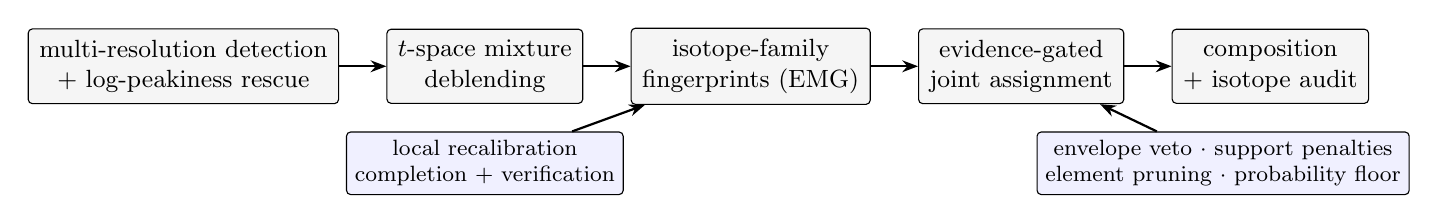
\begin{tikzpicture}[
  node distance=3.5mm and 6mm,
  stage/.style={draw, rounded corners=1.5pt, align=center, font=\small,
    inner sep=4pt, minimum height=9mm, fill=black!4},
  guard/.style={draw, rounded corners=1.5pt, align=center, font=\footnotesize,
    inner sep=3pt, fill=blue!6},
  arrow/.style={-{Stealth[length=2mm]}, thick},
]
\node[stage] (detect) {multi-resolution detection\\ + log-peakiness rescue};
\node[stage, right=of detect] (deblend) {$t$-space mixture\\ deblending};
\node[stage, right=of deblend] (family) {isotope-family\\ fingerprints (EMG)};
\node[stage, right=of family] (assign) {evidence-gated\\ joint assignment};
\node[stage, right=of assign] (out) {composition\\ + isotope audit};
\node[guard, below=of deblend] (recal) {local recalibration\\ completion + verification};
\node[guard, below=of out, xshift=-6mm] (guards) {envelope veto $\cdot$ support penalties\\ element pruning $\cdot$ probability floor};
\draw[arrow] (detect) -- (deblend);
\draw[arrow] (deblend) -- (family);
\draw[arrow] (family) -- (assign);
\draw[arrow] (assign) -- (out);
\draw[arrow] (recal) -- (family);
\draw[arrow] (guards) -- (assign);
\end{tikzpicture}
\end{adjustbox}
\caption{\rf{} stages. Raw events ($m/z$ list from
\texttt{.pos}/\texttt{.epos} or any spectrum source) flow left to right;
the parsimony guards (blue) are ablated individually in
Table~\ref{tab:ablation}.}
\label{fig:pipeline}
\end{figure}

\rf{} takes a raw event list --- big-endian \texttt{.pos}/\texttt{.epos},
or any array of $m/z$ values with optional positions --- and produces
ranged peaks, species assignments with per-candidate probabilities,
elemental and isotopic composition tables, audited isotope-ratio claims,
and (when positions are available) a spatial homogeneity analysis. The
stages are summarized below; every threshold named here is a configuration
key with the quoted default.

\subsection{Multi-resolution detection with a log-domain rescue channel}
Peaks are detected on histograms at several bin widths simultaneously
(0.001--0.02\,Da candidates, capped by a Freedman--Diaconis-derived
maximum), and the per-width detections are merged with
prominence-weighted clustering. Two detectors run per width: a standard
prominence detector on Savitzky--Golay-smoothed counts, and a
\emph{log-peakiness} detector that subtracts a median-filter baseline in
$\log_{10}$ space and scores candidates by prominence over local MAD noise
--- the channel that recovers low-amplitude peaks riding on thermal tails.
Detections seen at only one resolution are treated with suspicion
(shoulder suppression), one-sided tail artifacts are removed by a
valley test against the parent peak, and every surviving center is
re-estimated on the raw (unbinned) events by local density mode.

\subsection{Deblending in normalized time-of-flight space}
APT peak width is approximately constant in $t=\sqrt{m/z}$, so crowded
windows (peaks closer than 1.05\,Da spanning $\leq 6$\,Da) are re-fit as a
shared-width Gaussian mixture in $t$-space with a linear baseline, bounded
center offsets, and penalties on width drift. Fits that explain less than
half of the above-baseline signal are rejected in favor of the seed peaks
(a spike narrower than the width floor should not corrupt its neighbors),
and fitted areas replace histogram integrals only for the peaks in the
window.

\subsection{Isotope-family fingerprints with tail-aware fits}
For every plausible (element, charge) pair up to $4+$, \rf{} tries to
align the element's natural isotopologue ladder to the detected peaks. A
candidate family must (i) match its \emph{dominant} isotope, (ii)
reproduce natural relative abundances --- the fit is
area-parameterized so a shared exponential tail cannot silently reshape
fractions --- and (iii) beat competing families on a coherence-weighted
score. Three recovery mechanisms make this robust on real, imperfectly
calibrated data. A \emph{calibration-recovery tier} accepts
parts-per-thousand-scale shared shifts only under strong fingerprint
evidence. \emph{Family completion} lets a confirmed fingerprint claim
stragglers (including a wobbled dominant isotope) within a widened window
\emph{after} scoring, so completion can never buy a family its
acceptance. And \emph{member verification} handles the members blind
detection misses entirely: when a small isotope rides the thermal tail of
a large neighbor, its predicted (shifted) position is tested directly in
the raw event list as a local Poisson excess over the sideband baseline
--- the algorithmic version of ``if this is FeO, there must be a
$^{57}$FeO bump one dalton up; is there?'' Two-member families are
admissible only when the minor member's fitted fraction reproduces its
natural value tightly, a gate that is sharp exactly where plain
abundance coherence is not (it separates O$_2^+$, whose $+2$\,Da
satellite is 0.41\%, from S$^+$, whose $^{34}$S satellite is 4.2\%, on
the same miscalibrated peak). Confirmed families recenter their peaks
onto the reference mass scale, giving local recalibration for free.

\subsection{Molecular-family fingerprints}
The same machinery is applied to molecular series --- oxides,
dioxides, trioxides, dimers, nitrides, and carbides of the elements the
atomic pass anchored. This matters because molecular ions live at high
$m/z$ where calibration errors are largest, and they carry isotopologue
fingerprints just as distinctive as atomic families (FeO$^+$ inherits
Fe's $-2/+1/+2$\,Da satellite pattern). On a w\"ustite reference dataset
whose mass scale is off by $+40$--$80$\,mDa above 55\,Da, this pass is
the difference between reporting FeO and reporting a mixture of
Si$_2$O$^+$, Al$_2$O$^+$, and Fe$_2$S$^{2+}$ coincidences. Confirmed
molecular formulas are injected into the assignment candidate library
(even beyond its combinatorial atom-count cap) and boosted by a
fingerprint hint, mirroring atomic hints.

\subsection{Evidence-gated assignment with parsimony guards}
Candidate species (atomic and molecular, to 3 atoms and charge $4+$) are
scored per peak by mass agreement (Gaussian in a ppm-scaled window),
natural abundance, isotope-family consistency, charge priors, and
family-fingerprint hints, then resolved jointly: area-weighted support
maps for species, elements, and families feed back into the scores over
four iterations, so an assignment must be consistent with the whole
spectrum, not just its own peak. Softmax probabilities over the
per-peak candidates express residual ambiguity.

Candidates are physically constrained before scoring: an ion's charge
cannot exceed its atomic number (no H$^{2+}$), pure-hydrogen molecular
ions above charge 1 are excluded (H$_2^{2+}$ has no bound state and is
mass-degenerate with H$^+$, so admitting it silently multiplies the
hydrogen count), and noble-gas candidates carry a penalty because they
essentially never field-evaporate (He$^+$ at 4.0026\,Da is otherwise a
ready-made explanation for D$_2^+$ at 4.028 on deuterium-charged
specimens). On top of these, four parsimony guards --- the main
methodological contribution of this work --- prevent the failure mode
every combinatorial assigner is prone to, namely explaining real peaks
with chemically absurd species:

\begin{enumerate}
\item \textbf{Isotopologue-envelope veto.} A molecular candidate matched
through a \emph{minor} isotopologue is physical only if its dominant
isotopologue shows a correspondingly larger peak somewhere in the
spectrum ($\geq 25\%$ of the implied area). This mirrors, for molecules,
the dominant-isotope requirement that atomic families already obey. On a
SiO$_2$ control this single guard is what stops
$^{29}$SiH$_2^+$ ($m/z$ 31.998) from stealing 45\% of the O$_2^+$ peak at
31.995.
\item \textbf{Support-scaled element penalties.} Atomic candidates of
elements with no independent sample-level evidence are penalized on a
smooth ramp; molecular candidates pay per unsupported constituent.
Without this, the always-searched light elements (H, C, N, O, B, \dots)
capture charge-state peaks of the matrix on pure-metal spectra.
\item \textbf{Iterative element pruning.} After assignment, an element is
\emph{anchored} if it has an atomic rank-1 assignment at probability
$\geq0.35$, a confirmed family fingerprint, or a user hint; a
high-confidence molecular species may vouch for one unanchored partner if
all its other constituents are anchored (SiO$^+$ anchors O when Si is
anchored; an exotic N$_2$Ni$^{2+}$ anchors nothing). Unanchored elements
are removed from the library and assignment reruns --- the algorithmic
version of how an expert ranges: identify the element vocabulary first,
then explain every peak within it.
\item \textbf{Hydride-on-member guard.} An X-hydride candidate sitting a
few mDa from a member position of X's own confirmed isotope family is
the classic $+1$\,Da systematic, not independent chemistry; it pays a
penalty unless measured abundances actually deviate from the family's
natural pattern.
\end{enumerate}

Composition sums baseline-subtracted peak areas over assignment
probabilities, with a probability floor (5\%) and per-peak
renormalization so that losing candidates cannot siphon a few percent of
every strong peak into phantom elements. A parallel ``robust''
composition uses only high-confidence rank-1 assignments.

\subsection{Isotope audit and anomaly gating}
Every isotope-ratio claim is re-derived from raw events by a dual-shape
(Gaussian vs.\ exponentially modified Gaussian) family fit with explicit
interference components --- including single-hydride positions of the
major elements, the classic $+1$\,Da inflation source --- and anomaly
flags are downgraded unless the audit reproduces them, in the spirit of
\citet{london2019}: an anomaly claim must survive a model that is
\emph{trying} to explain it away. Counting-statistics $z$-scores carry a
systematic-error floor so that $10^5$-count peaks cannot manufacture
significance.

\subsection{Spatial segmentation}
When positions are available, voxelized local compositions are clustered
($k=2$--4) and extra regions are accepted only if they pass fraction,
composition-separation, silhouette, and spatial-contiguity gates; each
accepted region is then re-analyzed independently through the full
pipeline. Layered specimens thus report per-layer compositions instead of
a physically meaningless average.

\section{Benchmark design}
\label{sec:benchmark}

\subsection{Datasets}
\textbf{Synthetic ground truth.} Four synthetic specimens (1.5M events
each) with exact compositions, generated in normalized-TOF space with
realistic widths (MRP 800), 35\% one-sided thermal tails, and 2\% uniform
background: an Al--Mg--Si alloy, a Si/O oxide with molecular ions, a
Zn--Cu--Al alloy, and a layered Zn-on-Al specimen for segmentation. The
generator ships with \rf{}; every line position and intensity is known.

\textbf{Public reference data.} Eleven datasets, all CC-BY from Zenodo:
pure Si with Ni silicide (APAV's own example data), pure W at 18\,K, Ck10
low-carbon steel (Felfer), ODS ferritic steel (Wang), Mo--Hf alloy
(Leitner) from the FAIRmat collection \citep{zenodo7979668}; three
H/D-charged steel specimens with a shared expert range file
\citep{zenodo5534859}; FeO w\"ustite with exact 1:1 stoichiometry
\citep{zenodo10677562}; pure Li \citep{zenodo14848236}; and a (V,Al)N
nitride film with a shipped expert range file \citep{zenodo7788883}, which
adds a transition-metal nitride --- a chemistry outside the metals, steels,
and oxide of the rest of the set. Where a certified or nominal composition
exists we score against it; where an expert range file ships with the data
we score detection against its intervals and composition against the
range-file-applied reference. We also evaluated but \emph{rejected} a second
public FeO specimen (Zenodo 5838237): direct inspection showed oxygen nearly
absent from its spectrum and a large unranged peak at the $^{55}$ position,
so its nominal Fe:O${=}1{:}1$ label would have been false ground truth ---
a reminder that a dataset's stated chemistry must be verified against its
spectrum before it is trusted as truth.

\textbf{Out-of-domain spectra.} 120 MassBank records \citep{massbank2024}
--- curated, expert-annotated centroid lists for known organic compounds
--- rendered into semi-synthetic profile spectra with the same peak-shape
model as the synthetic APT data; and two real ToF-SIMS spectra in a
channel/mz/intensity text format \citep{zenodo15446699}, where recall is
scored on a reference list of known inorganic ions. Neither resembles APT
chemistry; both test whether the detector generalizes beyond the data the
pipeline was developed on.

\subsection{Comparators as stage ablations}
\label{sec:comparators}
Because no two of the open tools cover the same stage --- and none is a
fully unsupervised end-to-end pipeline (Sec.~\ref{sec:intro_gap}) --- a
head-to-head ``which tool is best'' framing would be a category error. We
therefore treat the comparators not as rival systems but as \emph{ablations
of individual stages of \rf{}}, which is also the fairest way to score them:
each is asked to do only the part it was built for.

\textbf{Detection front-ends (shared assigner).} pyOpenMS
\citep{rost2016openms}, ms\_deisotope, PyCCAPT \citep{monajem2025pyccapt},
and a na\"ive histogram-plus-sideband baseline all detect peaks but ship no
species assigner. We run each detector and hand its peak list to \rf{}'s
assignment stage, so their composition scores isolate \emph{detection}
quality under a fixed assigner. Section~\ref{sec:detection_ablation} makes
this an explicit ablation, adding the standard 1D mass-spectrum detectors
APT ranging never adopted --- CWT ridge lines, persistent homology, and
derivative zero-crossings --- against \rf{}'s own multi-resolution detector
and a naive prominence detector. Sharing \rf{}'s assigner can only help the
comparators, so this comparison is conservative against \rf{}.

\textbf{Independent quantifiers.} APAV's noise-corrected range
quantification \citep{smith2023apav} and APyT's spectrum-model fit bring
their own composition estimate given detected peaks or a fitted model; we
use it as-is. These ablate the \emph{quantification} stage rather than
detection. (APAV proper consumes user ranges; here it quantifies the
shared detected peaks, the closest automated use of it.)

The na\"ive baseline appears in both roles as a floor: it calibrates what
the shared assignment stage achieves with deliberately primitive detection.

\subsection{Metrics}
Composition: L1 distance to truth in atomic percent; \emph{fabricated
signal} (at.\% assigned to elements absent from the truth ---
the metric that punishes hallucination); largest major-element error;
top-element correctness. Detection: weighted line recall and peak
precision against exact synthetic lines; ion-weighted range recall
against expert range files; median absolute ppm mass error. Claims:
fabricated strong isotope anomalies on natural-abundance controls (the
correct count is zero). Cost: wall-clock runtime, single core.

\section{Results}
\label{sec:results}

Tables~\ref{tab:composition}--\ref{tab:foreign} are generated directly
from \texttt{outputs/benchmark/} by \texttt{scripts/build\_paper\_tables.py}.

\begin{table}[t]
\centering
\caption{Composition recovery: L1 distance to truth (at.\%, lower is
better; bold = best per dataset) with fabricated signal --- at.\%
assigned to elements absent from the truth --- in parentheses.
Truth sources: exact (synthetic), nominal composition, or expert
range file applied to the raw spectrum. Detector-only comparators
share \rf{}'s assignment stage (Sec.~\ref{sec:benchmark}); APAV and
APyT use their own quantification.}
\label{tab:composition}
\small
\begin{adjustbox}{max width=\textwidth}
\begin{tabular}{llrrrrrrr}
\toprule
Dataset & Truth & \rf{} & APAV & PyCCAPT & pyOpenMS & ms\_deisotope & APyT & na\"ive \\
\midrule
Syn.\ Al--Mg--Si & exact & \textbf{0.11} (0.00) & 0.12 (0.00) & 0.13 (0.00) & 10.44 (0.00) & 0.73 (0.00) & 3.44 (0.08) & 0.84 (0.00) \\
Syn.\ Si--O oxide & exact & 0.56 (0.00) & 0.90 (0.00) & 0.80 (0.00) & \textbf{0.53} (0.00) & 0.54 (0.00) & 15.62 (0.44) & 8.76 (0.00) \\
Syn.\ Zn--Cu--Al & exact & 0.84 (0.00) & 1.33 (0.00) & 1.08 (0.00) & \textbf{0.67} (0.00) & 0.67 (0.00) & 12.45 (4.07) & 17.95 (0.00) \\
Syn.\ Zn/Al layered & exact & 1.22 (0.00) & 4.97 (0.00) & 5.31 (0.00) & 0.86 (0.00) & \textbf{0.86} (0.00) & 21.35 (6.90) & 25.58 (0.00) \\
Pure W (18\,K) & nominal & \textbf{0.00} (0.00) & 9.01 (4.51) & 8.99 (4.49) & 22.56 (11.28) & 22.55 (11.28) & 21.33 (10.66) & 0.01 (0.00) \\
Ck10 steel & nominal & \textbf{2.64} (0.15) & 3.22 (0.05) & 3.18 (0.22) & 5.08 (0.29) & 5.41 (0.74) & 3.14 (0.48) & 4.23 (0.16) \\
ODS steel & range file & 5.10 (0.46) & 5.00 (0.41) & 5.59 (0.46) & 10.59 (1.03) & 14.75 (1.67) & \textbf{4.40} (0.45) & 5.59 (0.26) \\
Mo--Hf alloy & range file & \textbf{1.46} (0.11) & 2.93 (0.63) & 2.95 (0.64) & 16.98 (4.27) & 2.94 (0.59) & 2.09 (0.64) & 3.34 (0.99) \\
(V,Al)N nitride & range file & \textbf{16.69} (1.60) & 24.39 (9.28) & 23.16 (8.32) & 69.11 (33.53) & 68.49 (33.24) & -- & 23.78 (9.61) \\
FeO w\"ustite & nominal & \textbf{14.68} (0.24) & 100.00 (32.91) & 52.51 (26.10) & 44.34 (14.52) & 56.49 (22.64) & 139.78 (69.88) & 47.71 (16.76) \\
Pure Li & nominal & \textbf{0.00} (0.00) & 184.94 (92.47) & 0.01 (0.00) & 184.98 (92.48) & 0.00 (0.00) & 55.06 (27.53) & 182.12 (91.06) \\
H/D steel A & range file & \textbf{53.06} (8.46) & -- & 133.79 (29.94) & 66.87 (23.82) & 61.35 (10.98) & 69.55 (3.99) & 88.79 (25.44) \\
H/D steel B & range file & \textbf{13.26} (2.05) & 19.75 (4.47) & 20.37 (4.41) & 19.77 (5.51) & 13.63 (0.45) & 24.52 (2.74) & 19.59 (4.13) \\
H/D steel C & range file & 6.05 (0.82) & 10.14 (2.70) & 10.14 (2.71) & 6.39 (1.51) & \textbf{5.87} (0.00) & -- & 10.14 (2.73) \\
\midrule
Mean (n=11 complete) & & \textbf{3.62} & 30.20 & 9.17 & 28.80 & 10.78 & 27.56 & 28.70 \\
\bottomrule
\end{tabular}
\end{adjustbox}
\end{table}


\begin{table}[t]
\centering
\caption{Peak detection. Synthetic specimens: intensity-weighted
recall of known emitted lines, precision of detected peaks, and
median absolute mass error of matched lines. Public datasets with
expert range files: ion-weighted recall of reference ranges.
Bold = best per column.}
\label{tab:detection}
\small
\begin{tabular}{lrrrr}
\toprule
 & \multicolumn{3}{c}{Synthetic (exact lines)} & Range files \\
\cmidrule(lr){2-4}\cmidrule(lr){5-5}
Method & Recall$_w$ & Precision & $|\Delta m|$ (ppm) & Recall$_{ion}$ \\
\midrule
\rf{} & \textbf{1.000} & 0.984 & \textbf{2.2} & 0.997 \\
APAV & 1.000 & 0.974 & 168.2 & 0.998 \\
PyCCAPT & 1.000 & 0.974 & 165.0 & 0.991 \\
pyOpenMS & 0.991 & 0.688 & 94.1 & \textbf{0.999} \\
ms\_deisotope & 1.000 & \textbf{1.000} & 100.2 & 0.994 \\
APyT & 1.000 & 0.974 & 168.2 & 0.998 \\
na\"ive & 1.000 & 0.918 & 168.2 & 0.999 \\
\bottomrule
\end{tabular}
\end{table}


\begin{table}[t]
\centering
\caption{Detection ablation: only the peak detector is swapped; area
integration and \rf{}'s assignment stage are held identical, so scores
reflect detection alone. Columns: mean and worst-case composition L1
(at.\%) over the 14 datasets every detector completed, count of
catastrophic failures (L1$>$25\,at.\%), mean fabricated signal, and on
the synthetic specimens peak precision and median mass error. \rf{}'s
multi-resolution detector is the only one that never fails
catastrophically; its mass accuracy reflects raw-event centroiding and
family recentering that bin-apex detectors cannot match. Bold = best.}
\label{tab:detection_ablation}
\small
\begin{tabular}{lrrrrrr}
\toprule
Detector & mean L1 & worst L1 & \#L1$>$25 & fab. & Prec. & $|\Delta m|$ ppm \\
\midrule
\rf{} (multi-resolution) & \textbf{10.36} & \textbf{53.80} & 2 & \textbf{1.84} & \textbf{0.984} & \textbf{2.2} \\
Naive prominence & 28.51 & 184.93 & 4 & 10.63 & 0.959 & 113.9 \\
Savitzky--Golay prominence & 22.97 & 87.26 & 5 & 6.84 & 0.806 & 139.0 \\
CWT ridge lines & 30.90 & 184.93 & 4 & 11.99 & 0.963 & 113.9 \\
Persistent homology & 33.57 & 184.93 & 4 & 13.25 & 0.935 & 113.9 \\
Derivative zero-crossing & 23.76 & 81.12 & 5 & 7.64 & 0.867 & 139.0 \\
\bottomrule
\end{tabular}
\end{table}


\begin{table}[t]
\centering
\caption{Ablation: mean composition L1 and mean fabricated signal
(at.\%) over the nine ablation controls, plus two sentinel cases:
the Si--O oxide (molecular-ion apportionment) and pure W
(phantom-element suppression). Rows above the rule disable one
default stage (higher is worse); the two \texttt{++} rows re-enable
stages that are \emph{off} by default, showing they do not help.}
\label{tab:ablation}
\small
\begin{tabular}{lrrrr}
\toprule
Variant & mean L1 & mean fab. & Si--O L1 & W fab. \\
\midrule
Full pipeline (default) & 2.55 & 0.05 & 0.56 & 0.00 \\
-- family fingerprints & 7.99 & 3.51 & 0.62 & 0.00 \\
-- molecular-family recovery & 6.43 & 2.85 & 0.62 & 0.00 \\
-- element pruning & 7.46 & 2.34 & 0.56 & 12.01 \\
-- crowded-window deblending & 3.77 & 0.67 & 0.56 & 4.95 \\
-- probability floor & 2.70 & 0.05 & 0.56 & 0.00 \\
-- member verification & 2.52 & 0.05 & 0.56 & 0.00 \\
-- isotopologue-envelope veto & 2.74 & 0.03 & 0.56 & 0.00 \\
-- atomic support penalty & 5.18 & 1.09 & 0.56 & 0.00 \\
\addlinespace
++ log-peakiness channel (off by default) & 2.79 & 0.16 & 0.56 & 0.00 \\
++ family completion (off by default) & 2.55 & 0.05 & 0.56 & 0.00 \\
\bottomrule
\end{tabular}
\end{table}


\begin{table}[t]
\centering
\caption{Out-of-domain spectra. Left: 120 MassBank-derived
semi-synthetic profile spectra (organic fragment chemistry, exact
curated line lists). Right: real ToF-SIMS negative-polarity
spectra; recall on a reference list of known inorganic ions.
Bridge-based comparators are omitted here (in-process detectors
only).}
\label{tab:foreign}
\small
\begin{tabular}{lrrrr|rr}
\toprule
 & \multicolumn{4}{c|}{MassBank semi-synthetic} & \multicolumn{2}{c}{ToF-SIMS} \\
Method & Recall$_w$ & Precision & False pk & $|\Delta m|$ ppm & Ion recall & Peaks \\
\midrule
\rf{} & 0.980 & 0.994 & 0.0 & 82.1 & 1.000 & 156 \\
PyCCAPT & 0.974 & 0.979 & 0.1 & 95.5 & 1.000 & 128 \\
pyOpenMS & 0.974 & 0.573 & 2.9 & 78.9 & 1.000 & 148 \\
na\"ive & 0.994 & 0.874 & 0.5 & 106.6 & 1.000 & 172 \\
\bottomrule
\end{tabular}
\end{table}


\begin{table}[t]
\centering
\caption{Median wall-clock runtime (single process, Apple Silicon):
1.5M-event synthetic specimens and the 7.7M-event pure-W dataset.
Bridge methods (APAV, ms\_deisotope, APyT) include subprocess and
file I/O overhead.}
\label{tab:runtime}
\small
\begin{tabular}{lrr}
\toprule
Method & 1.5M events (s) & 7.7M events (s) \\
\midrule
\rf{} & 3.3 & 9.7 \\
APAV & 7.1 & 19.8 \\
PyCCAPT & 7.3 & 32.9 \\
pyOpenMS & 5.5 & 10.5 \\
ms\_deisotope & 7.5 & 27.4 \\
APyT & 350.5 & 59.9 \\
na\"ive & 5.6 & 17.9 \\
\bottomrule
\end{tabular}
\end{table}


\subsection{Reading the results}
Aggregated over the eleven datasets every method completed, \rf{}'s mean
composition error is 3.7\,at.\% L1 --- $2.4\times$ better than the best
comparator (PyCCAPT at 8.9, itself running \rf{}'s assignment stage) and
$8\times$ better than the independent quantifiers (APyT 27.6, APAV
30.3). The pattern behind the mean matters more than the mean: on clean
synthetic specimens all reasonable detectors agree to within a fraction
of an at.\% (differences there are noise), and the field separates
exactly where automated analysis is hard --- imperfectly calibrated real
data. On pure W, \rf{} reports 100.0\,at.\% W where comparators leave
9--23\,at.\% of phantom signal; on pure Li, three methods fabricate
$\sim$92\,at.\% of non-Li content while \rf{} reports lithium exactly;
on FeO w\"ustite, whose mass scale wobbles by $+40$--$80$\,mDa at high
$m/z$, \rf{} lands at the literature-typical APT oxide composition
(Fe$_{57}$O$_{43}$, the residual being the field's known oxygen deficit)
while every other method reports between 48 and 140 L1 --- APAV and APyT
assign the majority of the specimen to elements it does not contain.
\rf{} also correctly identifies the Ni-silicide contamination in APAV's
own Si example dataset, which the dataset's shipped range file does not
range.

Detection (Table~\ref{tab:detection}) shows the same shape: recall is
saturated for everyone on synthetic lines; the separators are precision
(\rf{} 0.984; only ms\_deisotope is comparable) and mass accuracy, where
family-fingerprint recentering puts \rf{} at 2.2\,ppm --- a $40\times$
margin over the best comparator (94\,ppm). The margin is structural: a
histogram apex on a thermally tailed peak sits several hundred ppm above
the true line, so any detector that reports apexes inherits that bias;
\rf{} measures the shared family shift and subtracts it.

\subsection{Detection ablation}
\label{sec:detection_ablation}
Table~\ref{tab:detection_ablation} isolates the detection stage directly:
we replace only the peak detector, hold area integration and \rf{}'s
assignment stage identical, and re-score. The baselines span the standard
1D mass-spectrum detectors the APT community never adopted --- naive and
Savitzky--Golay prominence, CWT ridge lines (the MassSpecWavelet family),
persistent homology, and derivative zero-crossings --- against \rf{}'s own
multi-resolution detector. This is the fair reading of the ``detector-only
comparator'' rows of Table~\ref{tab:composition}: those tools differ from
these baselines mainly in engineering, not in what a swapped detector can
buy under a fixed assigner.

Two findings stand out. First, on the easy majority the detectors are
close --- median L1 across detectors is $4.3$--$8.5$\,at.\% --- so on clean,
well-calibrated spectra the choice of detector is nearly immaterial, exactly
as one would expect. The means diverge because of \emph{catastrophic}
failures: naive, CWT, and persistent homology each fabricate ${\sim}92$\,at.\%
of non-lithium content on pure Li (they detect a background feature the
assigner then rationalizes), Savitzky--Golay smoothing merges the Si--O
molecular doublet into an L1 of 77, the derivative detector posts L1 $39$
on Mo--Hf, and on the (V,Al)N nitride the three scale-space detectors land
at L1 $66$--$72$ where \rf{} holds $16$. \rf{}'s multi-resolution detector
is the \emph{only} one with no catastrophic case (its worst is the
adversarial D-charged steel at L1 $54$, where every method struggles),
giving it a mean L1 of $10.4$ against $23$--$34$ for the alternatives --- a
$2$--$3\times$ margin attributable to detection alone, before any of the
assignment-stage parsimony guards that Table~\ref{tab:ablation} credits
separately. Second, the mass-accuracy gap
survives the ablation: every bin-apex detector clusters at
$110$--$140$\,ppm while \rf{} sits at $2.2$\,ppm, because raw-event
centroiding and family recentering are properties of \rf{}'s detector, not
its assigner.

The ablation (Table~\ref{tab:ablation}) identifies the load-bearing
stages: removing atomic family fingerprints costs $+5.4$ mean L1, element
pruning $+4.9$ (and 12\,at.\% of fabricated signal on pure W alone),
molecular-family recovery $+3.9$, the atomic support penalty $+2.6$, and
crowded-window deblending $+1.2$. The remaining guards show small marginal
effects \emph{in this configuration} because the defenses deliberately
overlap --- during development, before element pruning and molecular
recovery existed, the envelope veto alone was worth 20 L1 on the Si--O
control.

We also ran two stages the other way. Following the principle that a stage
should be kept only with evidence it helps, we tested two mechanisms that
earlier development had left enabled and found neither earned its place, so
both are now \emph{off} by default (the \texttt{++} rows of
Table~\ref{tab:ablation}). Re-enabling the log-peakiness rescue channel ---
a second detector meant to recover low-amplitude peaks on thermal tails ---
costs $+0.24$ mean L1 and improves weighted line or range recall on
\emph{no} dataset in the suite; on FeO it merely adds 17 peaks that inflate
L1 and fabricate signal. Re-enabling family completion (letting a confirmed
fingerprint claim stragglers in a widened window) changes no metric on any
dataset, because member verification and molecular-family recovery already
cover that failure mode. Removing both leaves the pipeline simpler, faster,
and slightly more accurate; the log-peakiness channel remains available as
an opt-in for anyone with a specimen where trace recall demonstrably helps.

Two honest failure readings. The D-charged steel specimens
(Table~\ref{tab:composition}, H/D rows) are adversarial for any
natural-abundance prior: the specimens were deliberately loaded with an
isotope that nature says should not be there, and although \rf{} still
posts the best or near-best score on all three, its absolute errors are
large --- an automated tool cannot know the experimenter enriched
deuterium unless told (\rf{} accepts element hints for exactly this).
And on the ODS steel, APyT's model fit beats \rf{} by 0.7 L1 against a
range-file reference that does not range the residual hydrogen \rf{}
reports; we note the gap rather than tune it away.

Finally, accuracy did not cost speed (Table~\ref{tab:runtime}). \rf{}
processes a 1.5M-event synthetic specimen in a median 3.3\,s and the
7.7M-event pure-W dataset in 9.7\,s single-core, making it the fastest of
the in-process methods --- below pyOpenMS (5.5\,s / 10.5\,s) despite doing
strictly more work (species identification, molecular-family recovery, and
composition rather than centroiding alone). The gain came from removing two
avoidable costs in the assignment stage: the per-candidate envelope score
over the ${\sim}$400k-entry species library was vectorized out of a
row-wise loop, and the combinatorial library, which is identical across the
element-pruning rounds, is now built once and reused. Neither change alters
any reported composition; both are pure implementation.

\section{Threats to validity}
\label{sec:threats}

\textbf{Development-set contamination.} The synthetic generator and the
five FAIRmat controls were used during \rf{}'s development; scores on
them are optimistic in the way any tool's self-reported scores are. Our
mitigations: the H/D steel, FeO, Li, MassBank, and ToF-SIMS datasets were
added \emph{after} the pipeline design was frozen and no thresholds were
tuned on them; and the entire harness is re-runnable by anyone on new
data with two commands.

\textbf{Shared assignment for detector-only tools.} Comparator
composition scores for PyCCAPT, pyOpenMS, ms\_deisotope, and the na\"ive
baseline measure detection differences under \rf{}'s assigner, because
those tools do not ship an assigner. This inflates their scores relative
to what a user of those tools alone could obtain --- the comparison is
conservative against \rf{}.

\textbf{Physics biases are shared.} APT undercounts O in oxides
\citep{gault2021primer}; on FeO every method inherits that bias, so we
report deviation from nominal stoichiometry knowing part of it is
physics, not algorithm. Detection efficiency, DC-field dissociation, and
multi-hit pileup corrections are out of scope for all compared tools.

\textbf{No public certified SRMs.} No open APT dataset of a certified
reference material exists; the nearest substitutes (stoichiometric
compounds, documented alloys) are what we use, and we state truth
sources per dataset.

\section{Related work}
Beyond the tools already discussed:
\citet{mikhalychev2020} rank candidate identities by Bayesian posterior;
\citet{wei2021patterns} classify isotope patterns with gradient-boosted
trees (CC BY-NC-ND licensed, 37-element vocabulary, admittedly weak on
monoisotopic species); \citet{meisenkothen2021} fit shared peak shapes
per channel and validate on certified uranium isotopics ---
the validation standard we would like the field to converge on;
\citet{wei2025automated} is the commercial CNN/LSTM effort. Relative to the
one open toolbox that also chains detection through composition ---
Felfer's semi-automated Atom-Probe-Toolbox
\citep{heller2024matlab,felfer_toolbox} --- \rf{} differs in being fully
unsupervised: it infers the element vocabulary from the spectrum rather
than requiring a user-supplied candidate list, has no interactive tuning
step, and performs no manual ion curation, so its operator variance is
exactly zero. Relative to the learned methods, every \rf{} stage is
inspectable configuration rather than trained weights, and it ships its own
falsification harness.

\section{Availability and reproduction}
\rf{} is pure Python (NumPy/SciPy/pandas), MIT-licensed, with the
benchmark harness, synthetic generator, control-download script, and
this paper's table generator included. Reproduction:
\texttt{scripts/download\_benchmark\_controls.sh} then
\texttt{scripts/run\_benchmark.py}; the MassBank, ToF-SIMS, and ablation
studies each have a dedicated script. Comparator versions and
environments are pinned in the repository.

\begin{thebibliography}{99}
\bibitem[APAV(2023)]{smith2023apav} J.~D.~Smith and M.~L.~Young,
``APAV: An open-source Python package for mass spectrum analysis in atom
probe tomography,'' \emph{J. Open Source Softw.} \textbf{8}(83), 4862
(2023). doi:10.21105/joss.04862.
\bibitem[Kühbach et al.(2021)]{kuhbach2021} M.~Kühbach, P.~Bajaj,
H.~Zhao, M.~H.~Çelik, E.~A.~Jägle, B.~Gault, ``On strong-scaling and
open-source tools for analyzing atom probe tomography data,'' \emph{npj
Comput. Mater.} \textbf{7}, 21 (2021).
\bibitem[Kühbach et al.(2022)]{kuhbach2022} M.~Kühbach et al.,
``Community-driven methods for open and reproducible software tools for
analyzing datasets from atom probe microscopy,'' \emph{Microsc.
Microanal.} \textbf{28}(4), 1038--1053 (2022).
\bibitem[Monajem et al.(2025)]{monajem2025pyccapt} M.~Monajem, B.~Ott,
J.~Heimerl, S.~Meier, P.~Hommelhoff, P.~Felfer, ``PyCCAPT: A Python
package for open-source atom probe instrument control and data
calibration,'' \emph{Microsc. Res. Tech.} \textbf{88}(12), 3199--3210
(2025).
\bibitem[Wilkinson et al.(2016)]{wilkinson2016fair} M.~D.~Wilkinson et al.,
``The FAIR Guiding Principles for scientific data management and
stewardship,'' \emph{Sci. Data} \textbf{3}, 160018 (2016).
\bibitem[Heller et al.(2024)]{heller2024matlab} M.~Heller, B.~Ott,
V.~Dalbauer, P.~Felfer, ``A MATLAB toolbox for findable, accessible,
interoperable, and reusable atom probe data science,'' \emph{Microsc.
Microanal.} \textbf{30}(6), 1138--1151 (2024).
\bibitem[Felfer et al.(2026)]{felfer_toolbox} P.~Felfer et al.,
``Atom-Probe-Toolbox,'' GPLv3 software repository, including
\texttt{massSpecFindPeaks}, \texttt{ionMatchPattern}, and
\texttt{rangeAutoEER},
\url{https://github.com/peterfelfer/Atom-Probe-Toolbox} (accessed 2026).
\bibitem[London(2019)]{london2019} A.~J.~London, ``Quantifying
uncertainty from mass-peak overlaps in atom probe microscopy,''
\emph{Microsc. Microanal.} \textbf{25}(2), 378--388 (2019).
\bibitem[Hudson et al.(2011)]{hudson2011} D.~Hudson, G.~D.~W.~Smith,
B.~Gault, ``Optimisation of mass ranging for atom probe microanalysis and
application to the corrosion processes in Zr alloys,''
\emph{Ultramicroscopy} \textbf{111}, 480--486 (2011).
\bibitem[Haley et al.(2015)]{haley2015guided} D.~Haley, P.~Choi,
D.~Raabe, ``Guided mass spectrum labelling in atom probe tomography,''
\emph{Ultramicroscopy} \textbf{159}, 338--345 (2015).
\bibitem[Gault et al.(2021)]{gault2021primer} B.~Gault et al., ``Atom
probe tomography,'' \emph{Nat. Rev. Methods Primers} \textbf{1}, 51
(2021).
\bibitem[Mikhalychev et al.(2020)]{mikhalychev2020} A.~Mikhalychev et
al., ``Bayesian approach to automatic mass-spectrum peak identification
in atom probe tomography,'' \emph{Ultramicroscopy} \textbf{215}, 113014
(2020).
\bibitem[Vurpillot et al.(2019)]{em2019} ``Enhancing element
identification by expectation--maximization method in atom probe
tomography,'' \emph{Microsc. Microanal.} \textbf{25}(2), 367--377 (2019).
\bibitem[Wei et al.(2021)]{wei2021patterns} Y.~Wei et al.,
``Machine-learning-enhanced time-of-flight mass spectrometry analysis,''
\emph{Patterns} \textbf{2}(1), 100192 (2021).
\bibitem[Meisenkothen et al.(2021)]{meisenkothen2021} F.~Meisenkothen,
D.~Samarov, M.~McLean, I.~Kalish, E.~B.~Steel, ``Adaptive peak fitting
for isotope analysis via atom probe mass spectrometry,'' \emph{Microsc.
Microanal.} \textbf{27}(S1) (2021).
\bibitem[Wei et al.(2025)]{wei2025automated} J.~Wei, R.~Ulfig,
D.~Reinhard, E.~Strennen, D.~J.~Larson, P.~M.~Voyles, ``Automated mass
spectrum labelling in atom probe tomography,'' \emph{Microsc. Microanal.}
\textbf{31}(S1), ozaf048.142 (2025).
\bibitem[Röst et al.(2016)]{rost2016openms} H.~L.~Röst et al., ``OpenMS:
a flexible open-source software platform for mass spectrometry data
analysis,'' \emph{Nat. Methods} \textbf{13}, 741--748 (2016).
\bibitem[FAIRmat(2023)]{zenodo7979668} M.~Kühbach et al., ``FAIRmat-NFDI
example datasets for atom probe microscopy,'' Zenodo record 7979668,
CC-BY-4.0.
\bibitem[Zenodo 5534859(2021)]{zenodo5534859} H/D-charged site-specific
steel specimens with shared range file, Zenodo record 5534859, CC-BY-4.0.
\bibitem[Zenodo 10677562(2024)]{zenodo10677562} Fe$_2$O$_3$/FeO/Fe$_3$O$_4$
atom probe datasets (LEAP-5000 XS), Zenodo record 10677562, CC-BY-4.0.
\bibitem[Zenodo 14848236(2025)]{zenodo14848236} Pure lithium atom probe
dataset, Zenodo record 14848236, CC-BY-4.0.
\bibitem[S\"alker et al.(2023)]{zenodo7788883} N.~S\"alker et al., dataset
for ``Computer vision assisted decomposition analysis of atom probe
tomography data'' ((V,Al)N and (Ti,Al)N nitride films with expert range
files), Zenodo record 7788883, CC-BY-4.0.
\bibitem[MassBank(2024)]{massbank2024} MassBank consortium,
``MassBank-data 2024.11,'' Zenodo record 14221628, CC-BY.
\bibitem[Zenodo 15446699(2025)]{zenodo15446699} ToF-SIMS spectra of
biofilm/planktonic/TSB samples in open text format, Zenodo record
15446699, CC-BY-4.0.
\end{thebibliography}

\end{document}
